\section{Benchmark}
Benchmarking this can be quite tricky since the time taken to find all possible solutions depends on not only the length of the pattern but also the number of unknowns. 

Figure 1 shows the time taken to find all possible solutions as the the length of the pattern goes up. This graph is adjusted for the number of unknowns. When adjusted for the number of unknowns in our graph, our tree traversal shenanigans should resemble an average-case binary tree traversal. Figure 1 shows a time complexity of $O(\log n)$ which matches our hypothesis.

\begin{figure}
    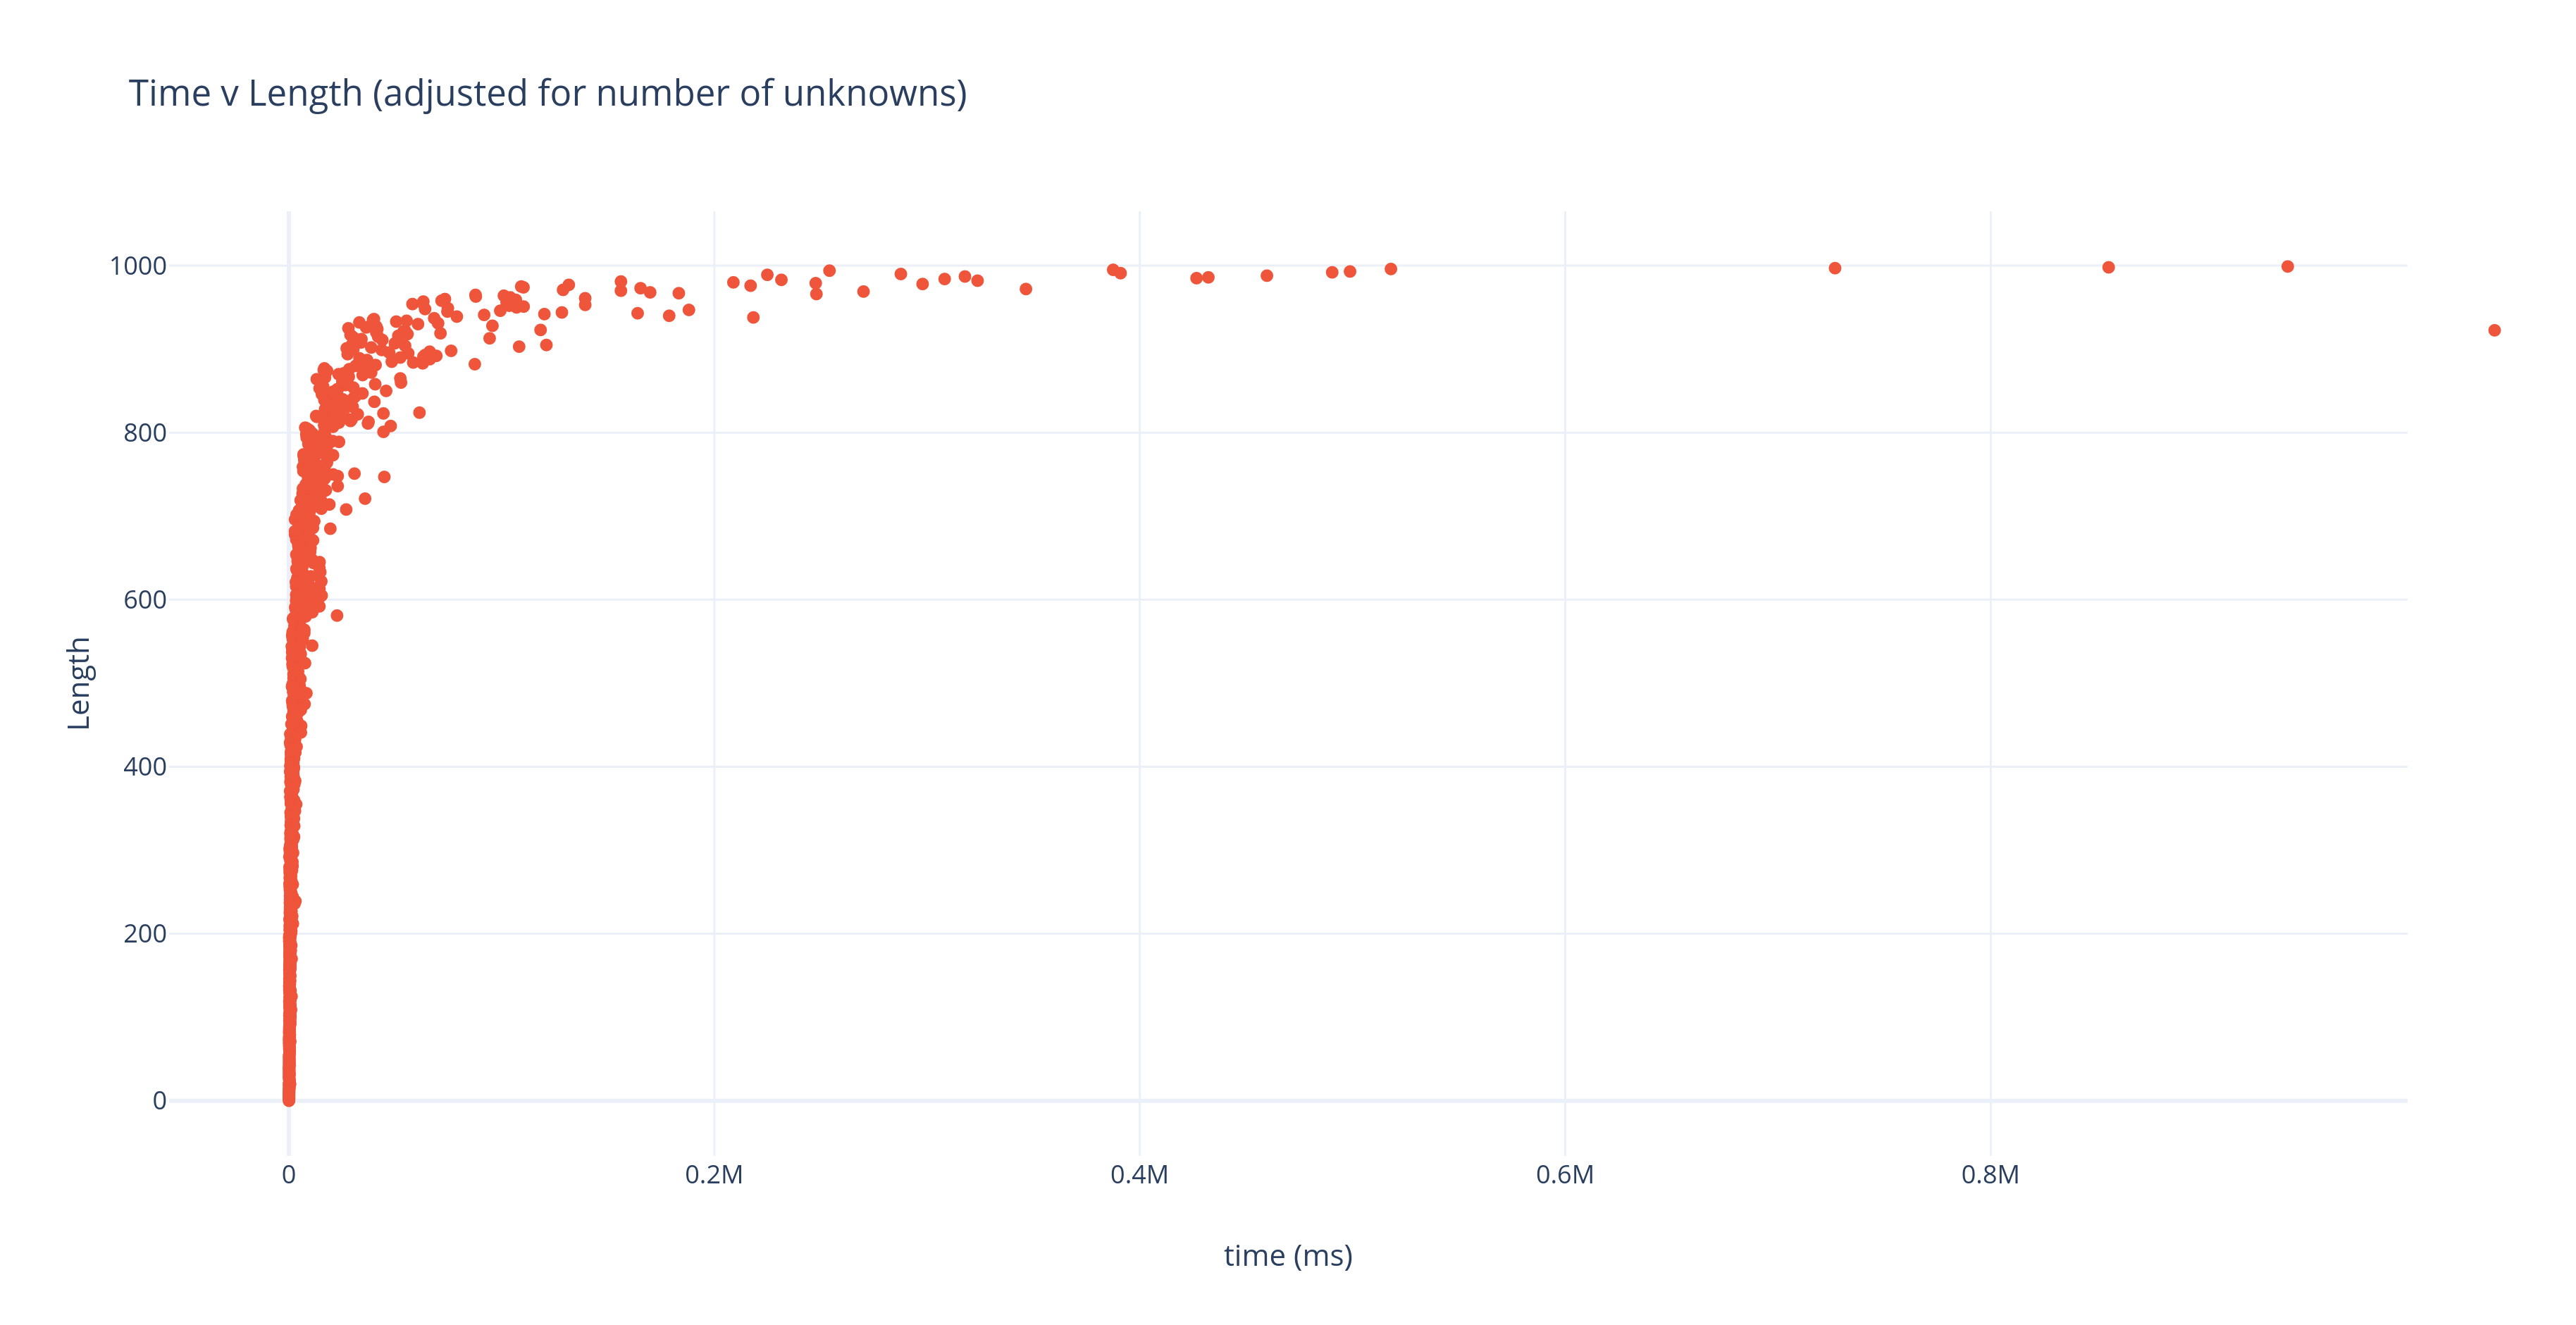
\includegraphics[width=\textwidth]{img/time_average}
    \caption{Graph, time taken vs length (adjusted for the number of unknowns)}
\end{figure}

Time taken to traverse the list will go up with the number of unknowns and the length of our pattern. 

But one thing is straight from our benchmark: which so many edge cases, pattern matching nightmares and no many broken hot springs, I have left my review on this resort.
\begin{figure}[bht!]
    \centering
    
\includegraphics[width=0.4\textwidth]{img/rating}
\end{figure}

Once again, the final version of the code can be found at \href{https://gist.github.com/ohshitnotgood/3ebf130cf0dab51544ba0ace3cec93ae}{this gist here}.